\documentclass[11pt,a4paper]{ctexart}
\usepackage[margin=1.8cm]{geometry}
\usepackage{amsmath,amssymb,bm}
\usepackage{booktabs,graphicx,xcolor,hyperref,array,float}
\hypersetup{colorlinks=true,linkcolor=blue,urlcolor=blue,citecolor=blue}
\setlength{\parindent}{2em}
\setlength{\parskip}{0.22em}
\newcommand{\norm}[1]{\left\lVert #1\right\rVert}
\newcommand{\R}{\mathbb{R}}
\title{IMU--UWB 状态增广与原始 TWR 联合 InEKF\\
共同时间戳校正与自适应捕获--跟踪两滤波器改进}
\author{共同 IMU/TWR 时延、增广捕获/重置与联合协方差跟踪}
\date{2026年8月3日}

\begin{document}
\pagestyle{plain}
\maketitle

\begin{abstract}
原状态增广方案采用
``IMU--InEKF $\rightarrow$ 世界系加速度 $\rightarrow$
LiftedRangeKF'' 松耦合级联。其独立辅助状态可扩大大初差捕获域，但
UWB 不能通过协方差交叉项修正姿态和 IMU 偏置，且末段容易受辅助状态
偏离物理流形影响。本文在不删除原捕获支路的前提下，增加使用原始 TWR
的 15 维联合 InEKF 跟踪支路。跟踪器的单个 Kalman 增益同时覆盖
姿态、速度、位置、陀螺偏置和加速度计偏置；因两个支路重复使用相同
IMU/UWB 且未维护滤波器间互协方差，不进行连续伪量测互灌，而由因果
监督器执行离散重置、切换和失效回退。

正式算法先经历 20 s 捕获/交叉协方差成熟期，随后在距离残差、拒绝率
及两支路一致性均通过时，以 $0.3$ 权重接入 tracker；持续健康证据经
10 s 低通、滞回和 1 s 保持后，tracker 权重在 5 s 内平滑升至 $1$。
5 s 宽限后若健康度仍低于 $0.27$，则平滑退回纯 capture 输出而不停止
后台 tracker。
此时增广支路退出稳态位置/速度输出，但继续在后台作为失锁监视和重置源。
该输出加权没有严格的融合协方差，属于明确标注的工程保护层。本轮按要求
不强制投影 $q,s,h$。独立标定表明同一日志行的 IMU 与 TWR 相对
OptiTrack 共同滞后约 $0.20$ s；实现统一校正二者的采集时刻，未只移动
UWB。TU Delft 12 条真实 TWR 日志、
零初差与 $[6,-6,3]^\top$ m 大初差组成 24 次配对回放；四项核心
指标均执行逐次无退化检查。普通六维距离 EKF 和原普通 TWR--InEKF
也在同一数据流中逐样本复现。结果表明：零初差时普通 InEKF 的全程
位置/速度中位数最好；大初差时新方法的全程位置中位数和均值最好并保持
12/12 收敛，但普通 EKF 的位置尾段仍更优。相对同实例 capture，四项
指标分别为 $24/0/0,22/2/0,24/0/0,22/2/0$ 次优/平/差。理想单锚点大初差蒙特卡洛
用于确认监督器不会牺牲原增广法的捕获能力。
\end{abstract}

\section{原松耦合方法及需要解决的问题}

原增广平移状态为
\begin{equation}
\chi=[q,s,h,p^\top,v^\top,1]^\top,\quad
q=\tfrac12p^\top p,\quad s=p^\top v,\quad h=v^\top v .
\end{equation}
对世界系加速度 $u$，其传播为
\begin{equation}
\chi_{k+1}^{-}=\Phi_L(u_k,\Delta t)\chi_k^+,\qquad
P_{L,k+1}^{-}=\Phi_LP_{L,k}^{+}\Phi_L^\top+Q_L ,
\end{equation}
而锚点 $a_i$ 的去偏半平方距离具有常观测行
\begin{align}
y_i&=\tfrac12\{(\rho_i^m-b_\rho)^2-\sigma_\rho^2\},\\
H_{L,i}&=
\begin{bmatrix}1&0&0&-a_i^\top&0_{1\times3}&
\tfrac12a_i^\top a_i\end{bmatrix}.
\end{align}
IMU 核心只为其提供
\begin{equation}
\hat u_w=\hat R(a_m-\hat b_a)+g.
\end{equation}
虽然接受 UWB 后会把 $\hat p_L,\hat v_L$ 同步到 IMU 核心的名义平移
状态，但并不更新 IMU 核心的姿态、偏置及交叉协方差。因此它仍是
\begin{equation}
\text{IMU--InEKF}\longrightarrow\hat u_w
\longrightarrow\text{LiftedRangeKF}
\end{equation}
的单向松耦合级联。

这一结构有两个互补特征：独立 $q,s,h$ 使量测行与位置估计无关，
大初差时不易遭遇普通距离线性化的门限锁死；但真实稳态中
$q-\frac12p^\top p$、$s-p^\top v$、$h-v^\top v$ 会受模型误差驱动
而偏离零流形，进而通过滤波器内部交叉协方差污染 $p,v$。若每次强制
投影则稳态可改善，却同时删除大初差捕获所依赖的独立辅助自由度。
因此，本次不以投影替换原方法，而是保留它作捕获/安全支路。

\section{共同 IMU--TWR 时间戳校正}

TU Delft 紧凑 CSV 的同一行包含 IMU、保持到下一次交易的八路 TWR
和 OptiTrack。只从 TWR 残差不能区分``UWB 相对 IMU 延迟''和
``机载传感器相对真值时间轴共同延迟''。加入旋转不变的 IMU 比力
模长证据后，采用后一种模型：
\begin{equation}
t_k^s=t_k^{\log}-\tau_s,\qquad \tau_s=0.20~\mathrm{s}.
\label{eq:common-delay}
\end{equation}
IMU 与 TWR 保持同一原始行配对，OptiTrack 则在采集时刻插值：
\begin{equation}
p_{\rm GT}^s(k)=
\operatorname{Interp}\!\left(
\{t_j^{\log},p_{\rm OT}(t_j^{\log})\},t_k^s\right).
\end{equation}
held TWR 的事件检测仍在原始日志上进行，随后才删除
$t_k^s$ 落在有效真值区间外的边界包。因而该操作不是只把 UWB 数组
前移若干行，也支持非整数采样周期的时延。

标定同时最小化两类独立分数。第一类在每个锚点内消去常偏差：
\begin{align}
e_{i,n}(\tau)&=\rho_{i,n}-
\norm{p_{\rm OT}(t_{i,n}^{\log}-\tau)-a_i},\\
J_\rho(\tau)&=
\sqrt{\frac{1}{N}\sum_{i,n}
\left(e_{i,n}(\tau)-\bar e_i(\tau)\right)^2}.
\end{align}
第二类利用
\begin{equation}
\norm{f_m(t)}
\approx
\frac{\norm{a_{\rm OT}(t-\tau)-g}}{\norm{g}}
\end{equation}
的旋转不变性，将两侧去均值、单位标准差后计算 RMSE。
预先指定的 triangle 标定日志得到 $J_\rho$ 与 IMU 分数的最优时延
分别为 $0.21$ s 和 $0.22$ s；按 held-range 事件和真值二阶差分的
可辨识精度固定取 $0.20$ s。其余 11 条日志的两类分数均 11/11 改善。

\begin{table}[H]
\centering
\small
\caption{共同时间校正的独立证据。}
\begin{tabular}{lrrr}
\toprule
指标 & 零延迟 & $0.20$ s & 扫描最优\\
\midrule
标定日志 TWR 去偏残差 RMSE & 0.17956 m & 0.15395 m & 0.21 s\\
标定日志 IMU/OptiTrack 标准化失配 & 1.45767 & 0.35076 & 0.22 s\\
12 日志 TWR RMSE 中位 & 0.18246 m & 0.15708 m & ---\\
12 日志 IMU 失配中位 & 1.35335 & 0.66570 & ---\\
\bottomrule
\end{tabular}
\label{tab:delay}
\end{table}

\begin{figure}[H]
\centering
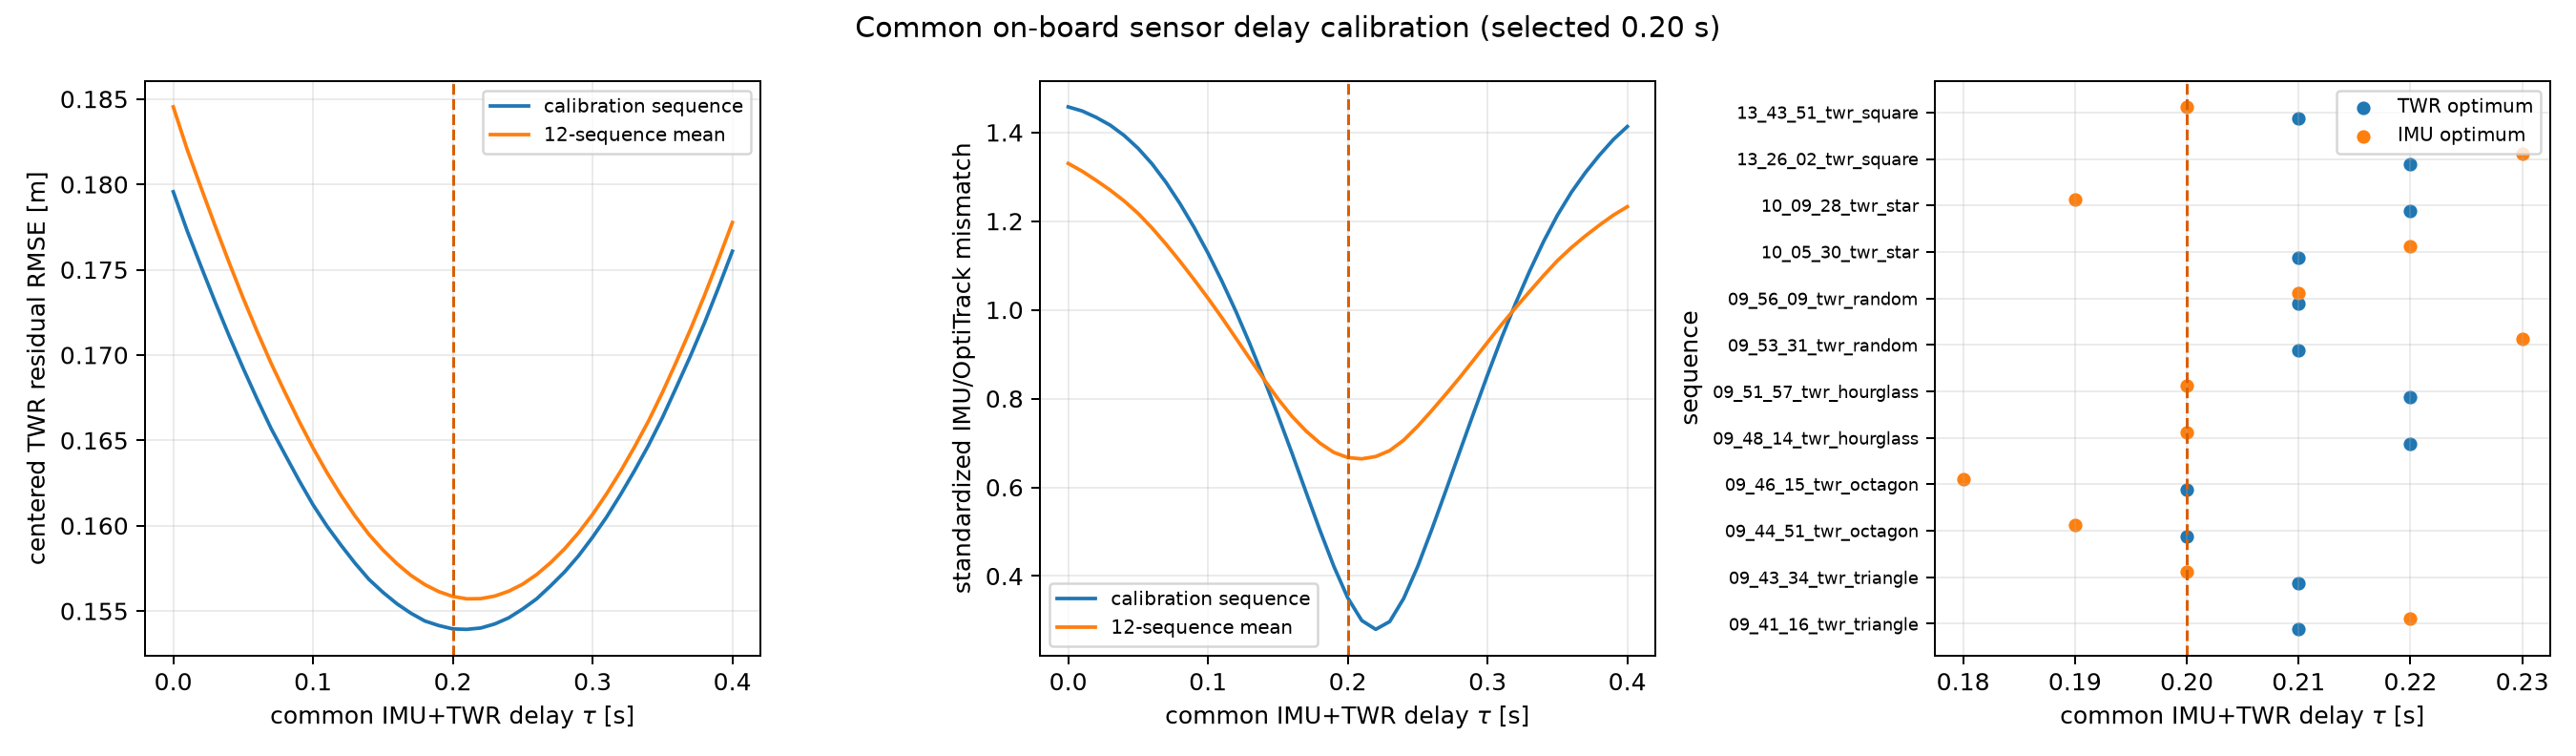
\includegraphics[width=0.98\textwidth]
{../imu-uwb-state-augment-deep-coupled-two-filters/results/time_alignment_calibration/time_alignment_diagnostic.png}
\caption{共同 IMU+TWR 时延扫描。虚线为正式采用的 $0.20$ s；左、中
分别为距离和 IMU 独立证据，右图给出每条日志的最优值。}
\label{fig:delay}
\end{figure}

式~\eqref{eq:common-delay} 解决当前离线回放/评价的时间轴。在线系统应
直接使用硬件采集时间；若只能在当前时刻收到属于 $t-\tau_s$ 的量测，
则需保存状态、协方差和 IMU，在测量时刻更新后重传播到当前时刻。
本 Python 回放未声称已经实现该固定延迟/OOSM 缓冲器。

\section{原始 TWR 联合 InEKF 跟踪支路}

\subsection{状态传播}

跟踪支路使用
\begin{equation}
X=
\begin{bmatrix}
R&v&p\\0&1&0\\0&0&1
\end{bmatrix}\in SE_2(3),\qquad
b=\begin{bmatrix}b_g^\top&b_a^\top\end{bmatrix}^\top ,
\end{equation}
误差顺序固定为
\begin{equation}
\delta x=
\begin{bmatrix}
\delta\theta^\top&\delta v^\top&\delta p^\top&
\delta b_g^\top&\delta b_a^\top
\end{bmatrix}^\top\in\R^{15}.
\end{equation}
名义传播为
\begin{align}
\dot{\hat R}&=\hat R(\omega_m-\hat b_g)^\wedge,\\
\dot{\hat v}&=\hat R(a_m-\hat b_a)+g,\qquad
\dot{\hat p}=\hat v,\\
\dot{\hat b}_g&=0,\qquad \dot{\hat b}_a=0,
\end{align}
协方差使用原 InEKF 的离散传播
\begin{equation}
P_{I,k+1}^{-}=\Phi_{I,k}P_{I,k}^{+}\Phi_{I,k}^\top+Q_{I,k}.
\end{equation}
关键区别是 $P_I$ 始终包含姿态、速度、位置和两类偏置之间的交叉块。

\subsection{原始距离 Kalman 更新}

正式数据的杆臂设为零。令
\begin{equation}
r_i=\rho_i^m-b_\rho,\quad
d_i=a_i-\hat p^-,\quad
\hat\rho_i=\norm{d_i},\quad
\nu_i=r_i-\hat\rho_i .
\end{equation}
代码先在左误差坐标构造位置方向行
\begin{equation}
\bar H_i=
\begin{bmatrix}
0_{1\times3}&0_{1\times3}&
d_i^\top/\hat\rho_i&
0_{1\times3}&0_{1\times3}
\end{bmatrix},
\end{equation}
再按当前 InEKF 误差定义转换为
\begin{equation}
H_i=\bar H_i\,
\operatorname{blkdiag}\!\left(
\operatorname{Ad}_{(\hat X^-)^{-1}},I_6\right).
\end{equation}
于是
\begin{align}
S_i&=H_iP_I^-H_i^\top+\sigma_\rho^2,\\
\operatorname{NIS}_i&=\nu_i^2/S_i,\qquad
K_i=P_I^-H_i^\top S_i^{-1},\\
\delta x_i&=K_i\nu_i .
\end{align}
通过门限后执行
\begin{align}
\hat X^+&=\operatorname{Exp}_{SE_2(3)}
(-\delta x_{i,1:9})\,\hat X^-,\\
\hat b^+&=\hat b^--\delta x_{i,10:15},\\
P_I^+&=(I-K_iH_i)P_I^-(I-K_iH_i)^\top
+K_i\sigma_\rho^2K_i^\top .
\end{align}
因此即使 $\bar H_i$ 的直接非零块只有位置，$K_i$ 的姿态、速度和偏置
行也可由传播形成的交叉协方差获得非零修正。这正是相对原松耦合
LiftedRangeKF 的``原始量测--全状态联合更新''。

\section{为什么不是连续互灌}

捕获器与跟踪器消费同一组 IMU 和 TWR。若把一个滤波器输出当成另一个
滤波器的独立伪量测，却不传播两滤波器之间的
\begin{equation}
P_{CT}=\operatorname{Cov}(\delta x_C,\delta x_T),
\end{equation}
同一信息会被重复计数，协方差通常过度自信。因此本实现不执行逐帧
双向 Kalman 伪量测，而采用三段式状态机：
\begin{enumerate}
\item \textbf{捕获：}原增广支路独立运行，跟踪器只在后台积累信息；
\item \textbf{跟踪：}联合 InEKF 健康时启用有界跟踪输出；
\item \textbf{回退：}联合支路不有限、分歧过大或量测统计恶化时，立即
      恢复到从未被覆盖的捕获输出。
\end{enumerate}

滚动窗口内定义
\begin{equation}
J_C=\sqrt{\frac1N\sum_{j=1}^N\nu_{C,j}^2},\quad
J_T=\sqrt{\frac1N\sum_{j=1}^N\nu_{T,j}^2},\quad
d_{CT}=\norm{\hat p_T-\hat p_C}.
\end{equation}
正式参数使用 $N=96$。为处理 capture 因未校正 IMU 偏置而漂移、但联合
tracker 仍被多锚量测明确支持的情况，再定义决定性量测优势
\begin{equation}
\mathcal D=\{n_{\rm anchor}\ge4\}\cap
\{f_{\rm rej,T}\le0.20\}\cap
\{J_T\le0.80~\mathrm m\}\cap
\{J_C-J_T\ge0.40~\mathrm m\}.
\label{eq:decisive-range}
\end{equation}
其中 $n_{\rm anchor}$ 是最近 96 次更新中的不同锚点数；故单锚点即使
径向残差很小也不能触发 $\mathcal D$。进入跟踪需同时满足
\begin{align}
t&>20~\mathrm{s}, &N_T&\ge64,\\
f_{\rm rej,T}&\le0.20,
&\bigl(d_{CT}&\le0.80~\mathrm{m}\ \text{或}\ \mathcal D\bigr),\\
J_T&\le0.80~\mathrm{m}, &J_T&\le J_C+0.08~\mathrm{m},
\end{align}
并连续保持 12 次更新。20 s 不是观测定理给出的常数，而是用于防止
范围拟合在少数锚点周期内过早乐观，使联合协方差及其交叉块有明确的
成熟期。

跟踪失效条件包括非有限状态、$d_{CT}>2.5$ m 且 $\mathcal D$ 不成立、
拒绝率超过 $0.45$，
或 $J_T>J_C+0.24$ m，连续 12 次后回退。在捕获期若跟踪器明显偏离，
且增广位置协方差已收缩，则执行离散重置
\begin{equation}
(\hat R_T,\hat v_T,\hat p_T,\hat b_T)
\leftarrow
(\hat R_C,\hat v_L,\hat p_L,\hat b_C).
\end{equation}
重置协方差保留捕获 IMU 核心的姿态/偏置主块以及增广滤波器的
$P_{vv},P_{pp},P_{vp}$，清零无法可靠获得的跨支路交叉块，并为位置、
速度分别加入 $0.75^2I_3$ 的膨胀项，再作对称化和特征值下限保护。
这是失效恢复的工程重置，不宣称等价于已知互协方差下的最优融合。

\section{持续健康度与自适应交接}

track 模式的布尔进入条件只表明 tracker 已可安全地以小权重参与，并不足以
证明它应全权接管。为此，令两支路预拟合距离 RMSE 为 $J_C,J_T$，定义
单位位置分歧上的距离拟合收益
\begin{equation}
\eta_k=
\frac{\max(J_C-J_T,0)}
{\max(d_{CT},d_0)},\qquad d_0=0.10~\mathrm{m}.
\end{equation}
当 $d_{CT}\le d_0$ 时距离证据分数取 1；否则将 $\eta_k$ 从
$0.03$ 到 $0.12$ 线性映射到 $[0,1]$。另由拒绝率、位置分歧、
绝对距离 RMSE 和相对距离 RMSE 构造四个下降型分数。当式
\eqref{eq:decisive-range} 成立时令位置分歧分数
$\gamma_{\rm disagree}=1$，否则仍由 $d_{CT}$ 下降映射。原始健康度为
\begin{equation}
\gamma_k=\min\{\gamma_{\rm reject},\gamma_{\rm disagree},
\gamma_{\rm abs},\gamma_{\rm rel},\gamma_{\rm evidence}\}\in[0,1].
\end{equation}
为避免单个锚点或短时 NLOS 使权重抖动，采用时间常数
$\tau_h=10$ s 的因果低通：
\begin{equation}
\bar\gamma_{k+1}=\bar\gamma_k+
\left(1-e^{-\Delta t/\tau_h}\right)(\gamma_k-\bar\gamma_k).
\end{equation}
当 $\bar\gamma\ge0.38$ 连续保持 1 s 时授权全 tracker 输出；授权后
只有 $\bar\gamma<0.25$ 才撤销，形成滞回。确认失锁不等待低通，直接
进入 capture 模式。

目标权重定义为
\begin{equation}
w^\star=
\begin{cases}
0,&\text{capture 模式},\\
1,&\text{track 模式且已全权授权},\\
0,&\text{track 已超过 5 s 且 }\bar\gamma<0.27,\\
0.3,&\text{其他 track 状态}.
\end{cases}
\end{equation}
实际 $w$ 受斜率限制：从 $0.3$ 到 $1$ 的上升斜率为
$0.7/5=0.14~\mathrm{s}^{-1}$，撤销授权时最多以
$1~\mathrm{s}^{-1}$ 回落。5 s 宽限保证刚切入时仍按要求从 $0.3$
开始，不会因为 10 s 低通状态尚未建立而立即退出；宽限后若持续证据
不足，则进一步回到 $w=0$，tracker 仍后台运行并可在健康恢复后重新参与。
输出为
\begin{equation}
\boxed{
\hat p_o=(1-w)\hat p_C+w\hat p_T,\qquad
\hat v_o=(1-w)\hat v_C+w\hat v_T .}
\end{equation}
因此健康 tracker 达到 $w=1$ 后，增广支路不再进入稳态位置/速度输出，
只继续作为初始化、失锁捕获、健康监视和离散重置源。姿态和偏置在 track
模式取联合 InEKF 支路。本轮不强制投影 $q,s,h$；它们的流形偏离问题没有
被删除，而是通过稳态退出输出降低影响。

由于没有 $P_{CT}$，实现不输出声称严格一致的 $P_o$；若下游必须使用
一致协方差，后续应增加交叉协方差传播或协方差交集，而不能把两者当作
独立估计。

本设计借鉴 Sifour--Berkane--Tayebi 的级联紧耦合思想，但没有照搬
其观测器。对方使用单 UWB 距离、IMU 和已知惯性方向的体坐标向量
（如磁力计），由重力方向与第二个向量重构完整姿态，并在其假设下证明
AGAS。本数据有 8 个绝对位置锚点，几何约束更丰富；却没有磁力计提供的
独立体坐标航向方向，而且存在 IMU 偏置、TWR 偏置/NLOS 和随机门限。
因此多锚点 TWR 可通过运动产生的交叉协方差间接修正姿态/偏置，却不能
替代磁力计的瞬时航向信息，也不能继承其 AGAS 证明。

\section{验证结果}

\subsection{自动测试}

共 28 项测试全部通过，覆盖原状态增广数值一致性、捕获支路逐元素等同
于原松耦合滤波器、$0.3\rightarrow1$ 平滑交接、低健康
$0.3\rightarrow0$ 保护、重置协方差对称半正定、健康授权与非有限
状态回退、共同时间校正保持 IMU/TWR 配对、TWR 与 IMU 两类独立时延
证据、决定性优势必须至少四锚、capture-only 合成时长拒绝、合成输出
非平凡激活，以及 30 s 真实大初差四指标无退化回归。基线测试把普通 EKF 和
普通 InEKF 的完整位置/速度时序逐元素与原 Task06 运行函数比较，
两条基线完全一致。测试入口为
\begin{verbatim}
.\run_deep_coupled.ps1 -Mode test
\end{verbatim}

\subsection{12 条真实日志配对批测}

数据使用 TU Delft UWB dataset v1 的 12 条 TWR 日志。每条分别从
零位置偏差和 $[6,-6,3]^\top$ m 偏差开始，共 24 次。松耦合对照不是
另一次独立运行，而是同一个估计器内部从未被 tracker 改写的 capture
支路；因此两者的 IMU、UWB、事件顺序和数值噪声完全相同。
所有真实方法共同采用式~\eqref{eq:common-delay} 的 $0.20$ s 时间校正。
此外，同步运行普通六维原始距离 EKF 和原 Task06 普通 TWR--InEKF：
前者使用相同世界系加速度和 64 次 gate 预热；后者使用相同原始
IMU/TWR，立即启用 gate、没有捕获重置。新增 tracker 与普通 InEKF
同为 15 维联合更新，但 tracker 具有 128 次预热及失配后的捕获重置。

\begin{table}[H]
\centering
\scriptsize
\setlength{\tabcolsep}{3.2pt}
\caption{24 次真实回放汇总。三列方法值为合并中位数；两列差值为
逐次配对差值的中位数。}
\begin{tabular}{lrrrrr}
\toprule
指标 & 松耦合增广 & deep 未校正 & deep 已校正 & 已校正 deep & 已校正 deep\\
 & $\tau_s=0.20$ & $\tau_s=0$ & $\tau_s=0.20$ & $-$松耦合 & $-$未校正 deep\\
\midrule
全程位置 RMSE (m) & 0.386090 & 0.368936 & 0.338625 & $-0.020030$ & $-0.028444$\\
末 5 s 位置 RMSE (m) & 0.312664 & 0.237738 & 0.211746 & $-0.092643$ & $-0.023142$\\
全程速度 RMSE (m/s) & 0.518496 & 0.506414 & 0.490124 & $-0.038338$ & $-0.036507$\\
末 5 s 速度 RMSE (m/s) & 0.521877 & 0.482974 & 0.379749 & $-0.075905$ & $-0.127923$\\
\bottomrule
\end{tabular}
\label{tab:real}
\end{table}

已校正 deep 相对同时间轴松耦合的逐次优/平/差依次为
$24/0/0,22/2/0,24/0/0,22/2/0$；相对当前同算法但未校正时间戳的
deep 则为 $23/0/1,22/0/2,20/0/4,20/0/4$。因此 $0.20$ s 校正改善
了四项总体中位数，但不保证每条轨迹都单调改善。

\subsubsection{普通 EKF、普通 InEKF 与五方法对比}

下表的``联合 tracker''专指所提估计器内部原始 TWR 联合 InEKF
支路的独立输出：
\begin{equation}
\hat p_{\rm tr}=X_{\rm tr}[1\!:\!3,5],\qquad
\hat v_{\rm tr}=X_{\rm tr}[1\!:\!3,4].
\end{equation}
它维护姿态、速度、位置、陀螺偏置和加速度计偏置的同一个 15 维协方差，
所以原始距离创新可经交叉协方差联合修正这些量；它又会由 capture 离散
重置并使用 128 次 gate 预热。该行既不是普通 InEKF 基线，也不是最终
输出。表中的``自适应输出''才是
$\hat p=(1-w)\hat p_{\rm cap}+w\hat p_{\rm tr}$（速度同理），其中
$w$ 由健康监督器在 $0$、$0.3$ 和 $1$ 之间平滑调整。

\begin{table}[H]
\centering
\scriptsize
\setlength{\tabcolsep}{3.2pt}
\caption{五方法真实批测。位置单位为 m，速度单位为 m/s；均为 12 条
日志的统计。}
\begin{tabular}{llrrrrrr}
\toprule
初值 & 方法 & 全程位置中位 & 全程位置均值 & 末段位置中位 &
全程速度中位 & 末段速度中位 & 收敛\\
\midrule
nominal & 普通 EKF & 0.366288 & 0.368687 & \textbf{0.160536} &
0.503423 & 0.385034 & 12/12\\
nominal & 普通 InEKF & \textbf{0.322048} & 0.353685 & 0.162547 &
\textbf{0.310763} & \textbf{0.322776} & 12/12\\
nominal & 松耦合增广 & 0.379737 & 0.372251 & 0.312664 &
0.518496 & 0.521877 & 12/12\\
nominal & 联合 tracker & 0.330571 & 0.354370 & 0.163200 &
0.347541 & 0.323892 & 12/12\\
nominal & 自适应输出 & 0.331862 & \textbf{0.349604} & 0.211725 &
0.490102 & 0.379651 & 12/12\\
\midrule
large & 普通 EKF & 0.460327 & 0.460873 & \textbf{0.160536} &
1.315530 & 0.385034 & 12/12\\
large & 普通 InEKF & 0.551103 & 84.233855 & 0.369452 &
0.873325 & 0.438903 & 7/12\\
large & 松耦合增广 & 0.386254 & 0.384465 & 0.312664 &
0.521700 & 0.521877 & 12/12\\
large & 联合 tracker & 0.426331 & 0.428299 & 0.165255 &
0.711201 & \textbf{0.324157} & 12/12\\
large & 自适应输出 & \textbf{0.356247} & \textbf{0.362371} & 0.211746 &
\textbf{0.490124} & 0.379749 & 12/12\\
\bottomrule
\end{tabular}
\label{tab:all-real}
\end{table}

零初差时，普通 InEKF 的全程位置、全程速度和末段速度中位数最好，
普通 EKF 的位置尾段最好；自适应输出的全程位置均值最低。大初差时，
自适应输出的全程位置中位数、均值和全程速度中位数最好，
且为 12/12 收敛；普通 InEKF 只有 7/12 收敛，最严重运行全程/末段
位置 RMSE 达 $493.138/832.187$ m，最多拒绝 15475 次量测。联合
tracker 通过预热/重置保持 12/12，其最大全程位置为 $0.623$ m；
自适应输出的 24 次最大全程位置 RMSE 为 $0.4885$ m。

全部 24 次中，自适应输出相对普通 EKF 的全程位置、末段位置、全程
速度和末段速度分别优于 $19,8,20,10$ 次；相对普通 InEKF 分别为
$12,9,9,7$ 次（两个末段指标各另有 3 次相同）。因此，本方法
的优势是大初差全程位置鲁棒性和相对松耦合的全面改善，不是所有稳态
指标都超过普通滤波器。24 次运行中有 10 次实际达到 $w=1$，8 次在
结束时仍为 $w=1$；说明全权接管确实发生，但不会对证据不足的轨迹
强制执行。

第一次启用正确时间轴、尚未加入低健康输出保护时，square 13\_26 的
nominal/large 末 5 s 位置相对 capture 各退化约 $0.01005$ m。
该失败结果保留在
\texttt{results/deep\_coupled\_delay\_pre\_health\_guard}。
加入 $\bar\gamma<0.27$ 保护后，两次均回到与 capture 相同，最终四项
验收全部零退化。

\subsubsection{同算法的零延时假设自对照}

原文的``同行即时生效版本''是一个含糊说法，原意是把同一 CSV 行的
IMU/TWR 当作在日志时刻立即采集，即
$t_k^{\rm acquisition}=t_k^{\rm log}$、$\tau_s=0$；它不是另一种
Kalman 更新，也不表示真实系统没有计算延迟。进一步核查发现，原先引用的
\texttt{results/deep\_coupled\_full} 还缺少后来加入的低健康保护和
决定性距离优势逻辑，因此旧表把算法版本变化与时间戳变化混在了一起。
本表已改为用当前完全相同的 deep 代码和参数重放 24 次，仅改变
$\tau_s=0$ 或 $0.20$ s；``优/平/差''按已校正相对未校正逐次判定：
\begin{table}[H]
\centering
\small
\caption{当前同一 deep 算法在共同时间戳校正前后的自对照。}
\begin{tabular}{lrrrr}
\toprule
指标 & 未校正 $\tau_s=0$ & 已校正 $\tau_s=0.20$ & 相对变化 & 优/平/差\\
\midrule
全程位置 RMSE & 0.368936 m & 0.338625 m & $-8.2\%$ & 23/0/1\\
末 5 s 位置 RMSE & 0.237738 m & 0.211746 m & $-10.9\%$ & 22/0/2\\
全程速度 RMSE & 0.506414 m/s & 0.490124 m/s & $-3.2\%$ & 20/0/4\\
末 5 s 速度 RMSE & 0.482974 m/s & 0.379749 m/s & $-21.4\%$ & 20/0/4\\
\bottomrule
\end{tabular}
\label{tab:delay-filter}
\end{table}
四个总体中位数均改善，但不是每条日志都改善。正确时间戳是物理模型
修正，不是保证任意滤波器、任意初值的经验指标单调下降的调参；普通
InEKF 的立即门限在大初值下仍可能因初段创新变化而锁死。

\begin{figure}[H]
\centering
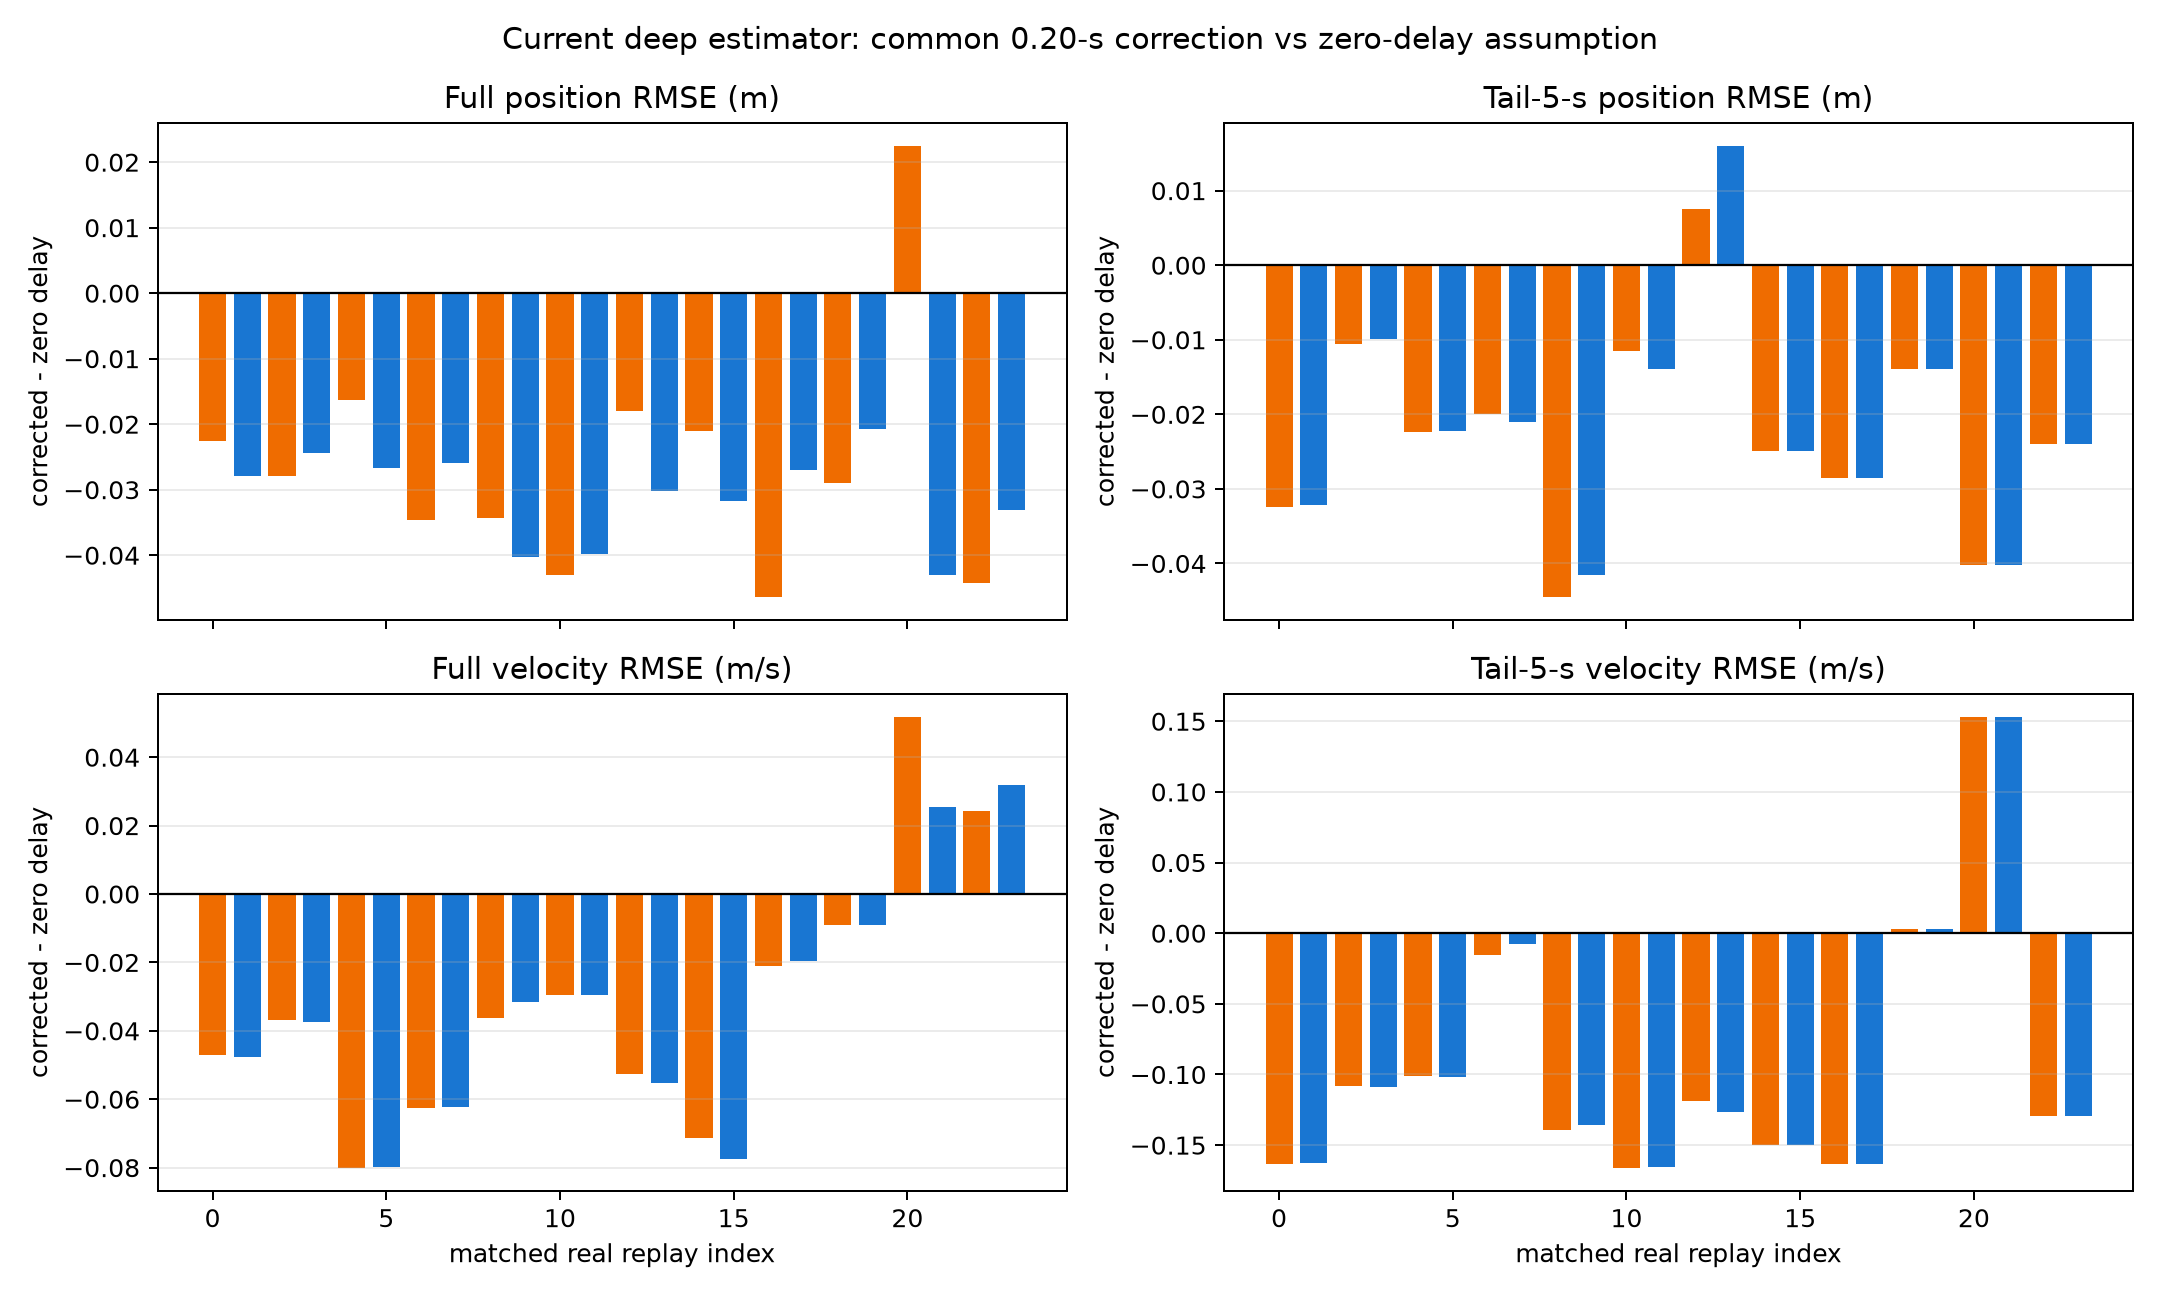
\includegraphics[width=0.98\textwidth]
{../imu-uwb-state-augment-deep-coupled-two-filters/results/deep_coupled_time_alignment_self_comparison/paired_deltas.png}
\caption{当前同一 deep 算法的 24 次时间戳自对照。纵轴为
$0.20$ s 校正减零延时假设；负值表示校正后误差更小。相邻橙/蓝柱为
同一日志的 large/nominal 初值，不隐藏少量正差值。}
\label{fig:deep-delay-self-comparison}
\end{figure}

\begin{figure}[H]
\centering
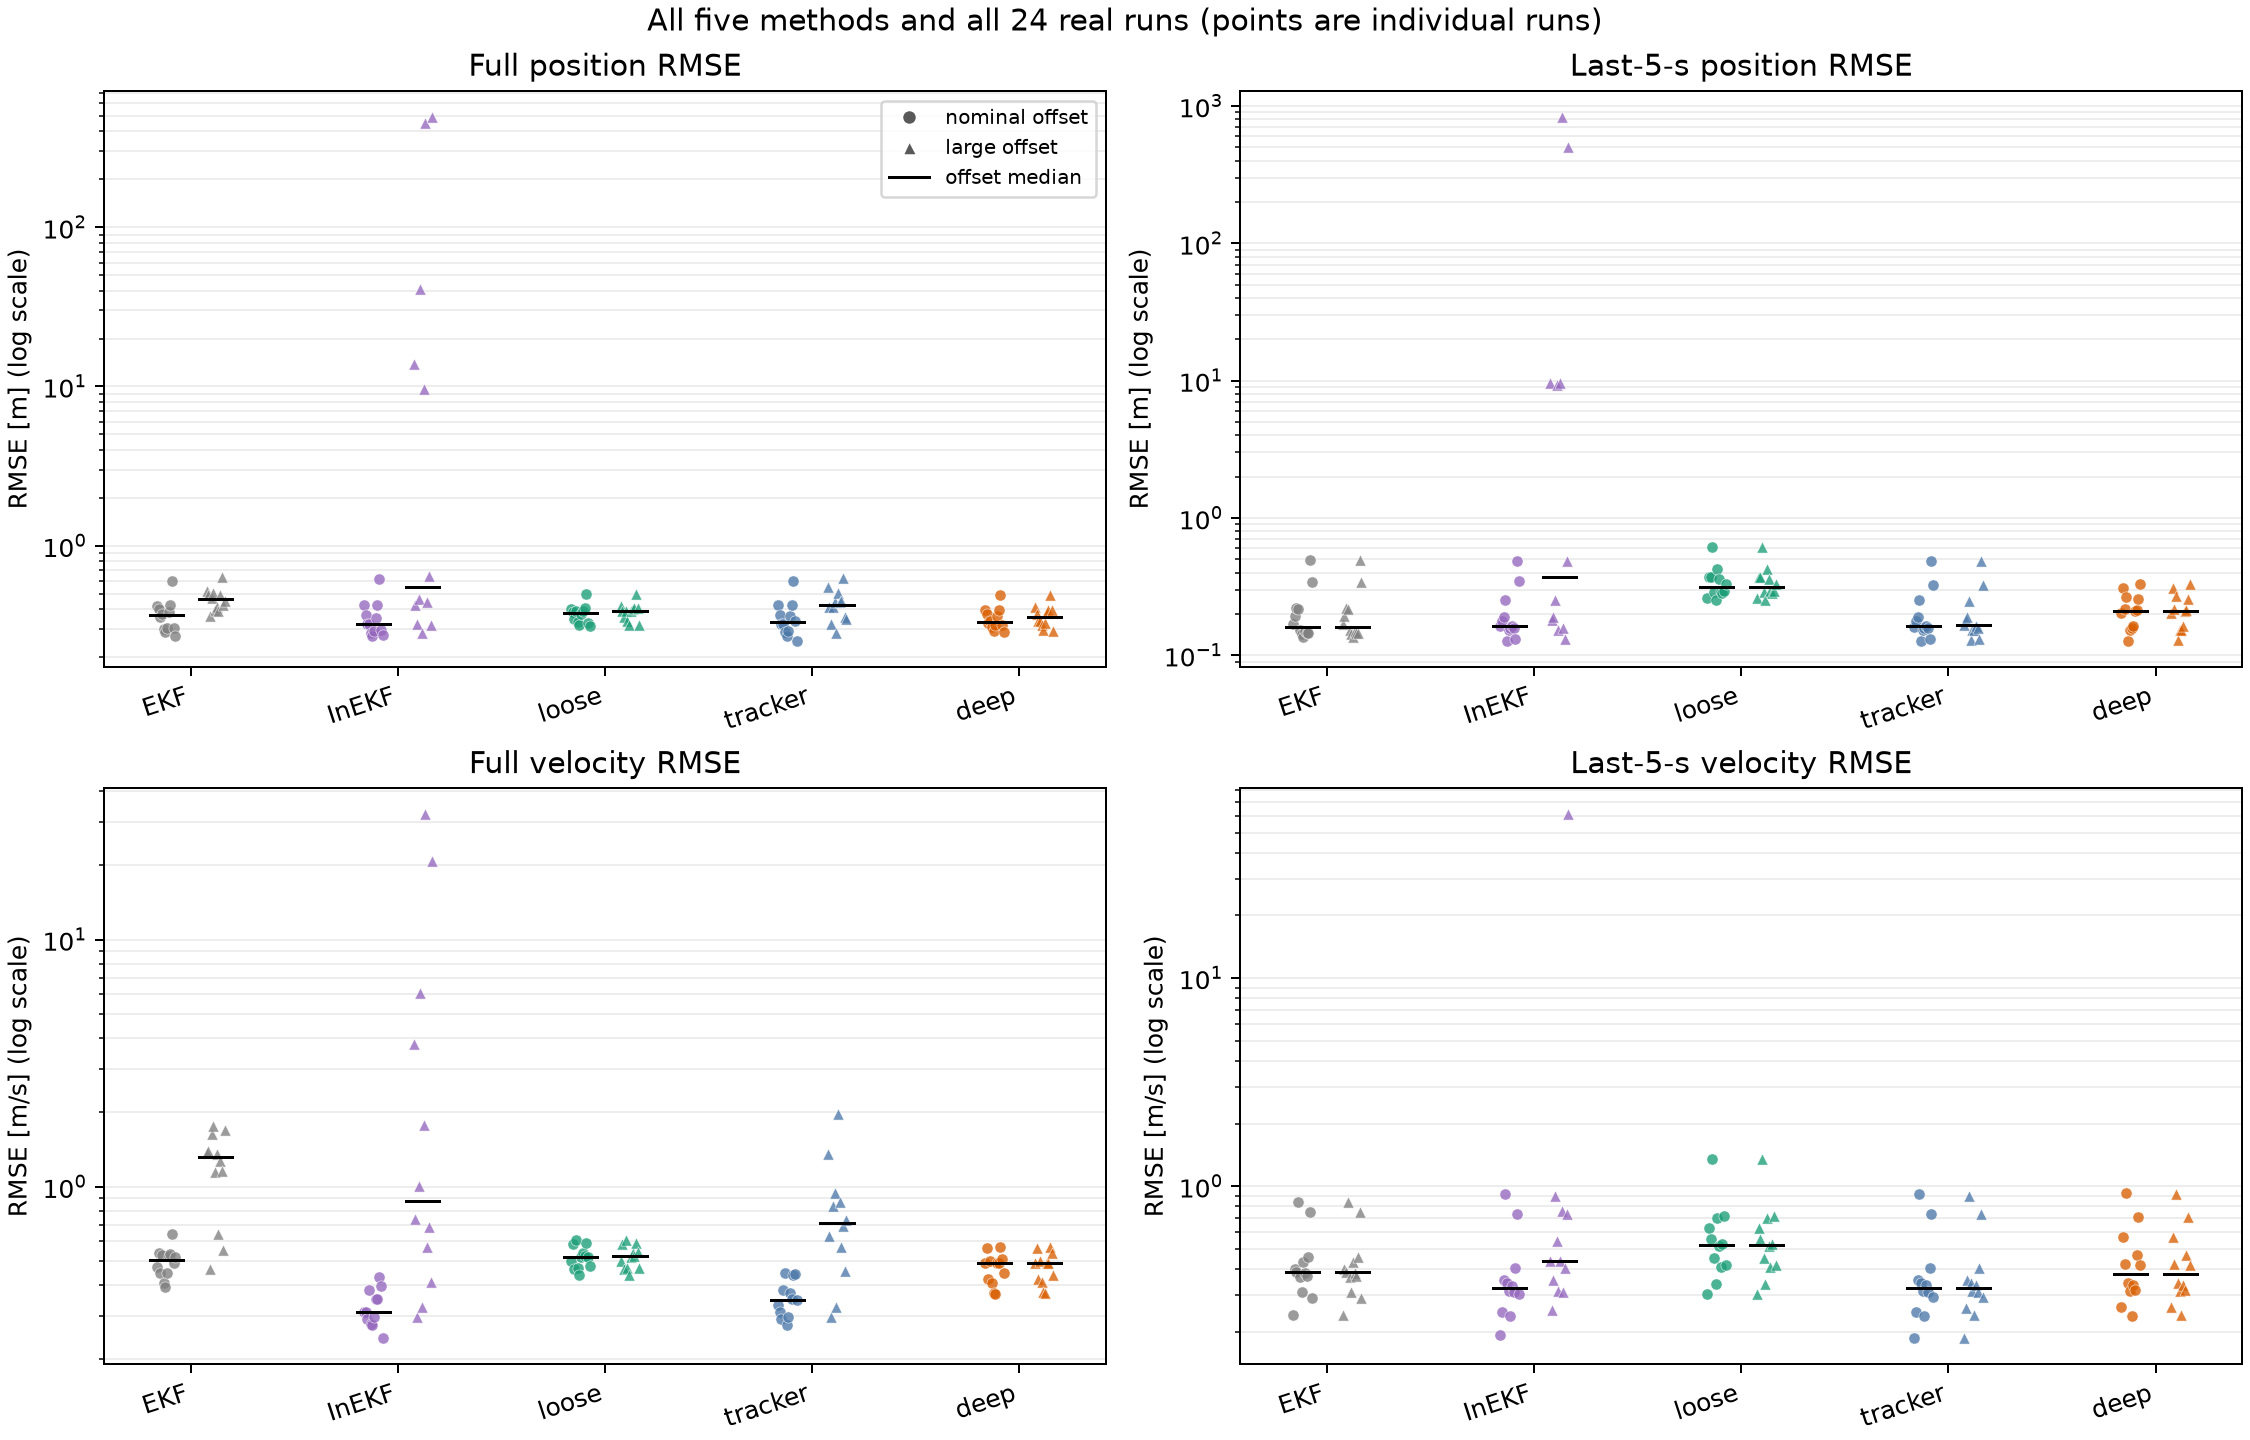
\includegraphics[width=0.98\textwidth]
{../imu-uwb-state-augment-deep-coupled-two-filters/results/deep_coupled_delay_full/real/all_methods_comparison.png}
\caption{五方法全部 24 次运行。圆点/三角分别为 nominal/large 初值，
黑横线为各初值中位数；对数纵轴完整保留普通 InEKF 和联合 tracker
的大初差离群值。}
\label{fig:all-methods}
\end{figure}

\begin{figure}[H]
\centering
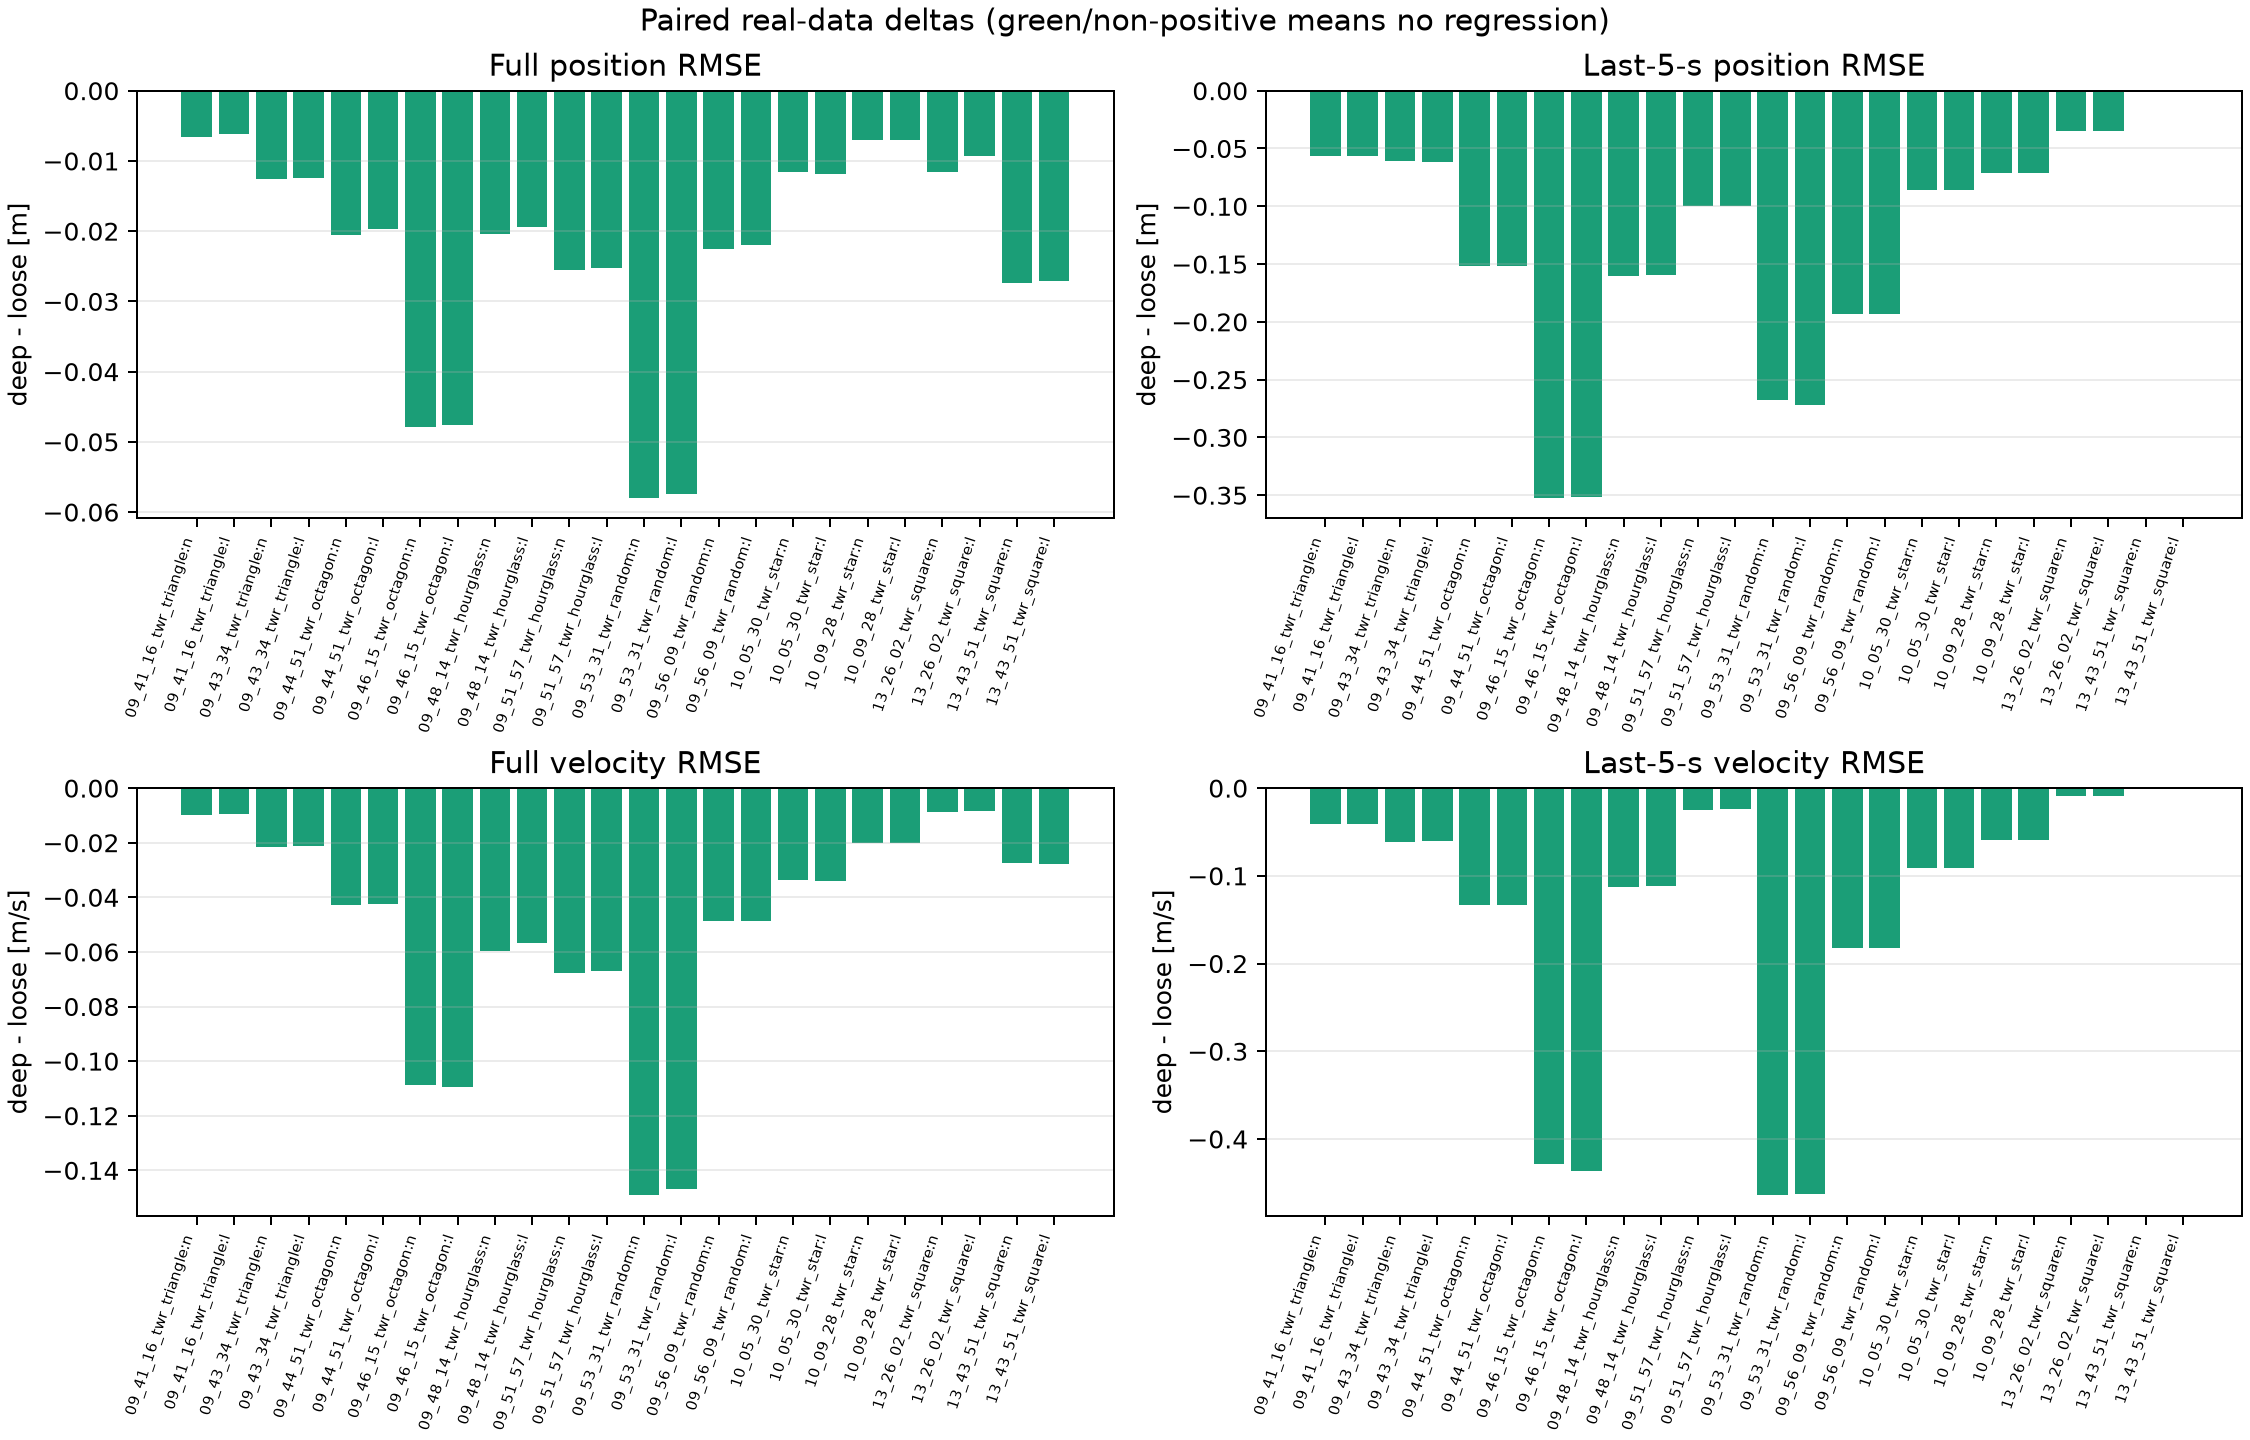
\includegraphics[width=0.98\textwidth]
{../imu-uwb-state-augment-deep-coupled-two-filters/results/deep_coupled_delay_full/real/paired_deltas.png}
\caption{24 次真实回放的逐次配对差值。纵轴为改进减松耦合，非正表示
不退化；图中不裁掉任何轨迹。}
\label{fig:deltas}
\end{figure}

\begin{figure}[H]
\centering
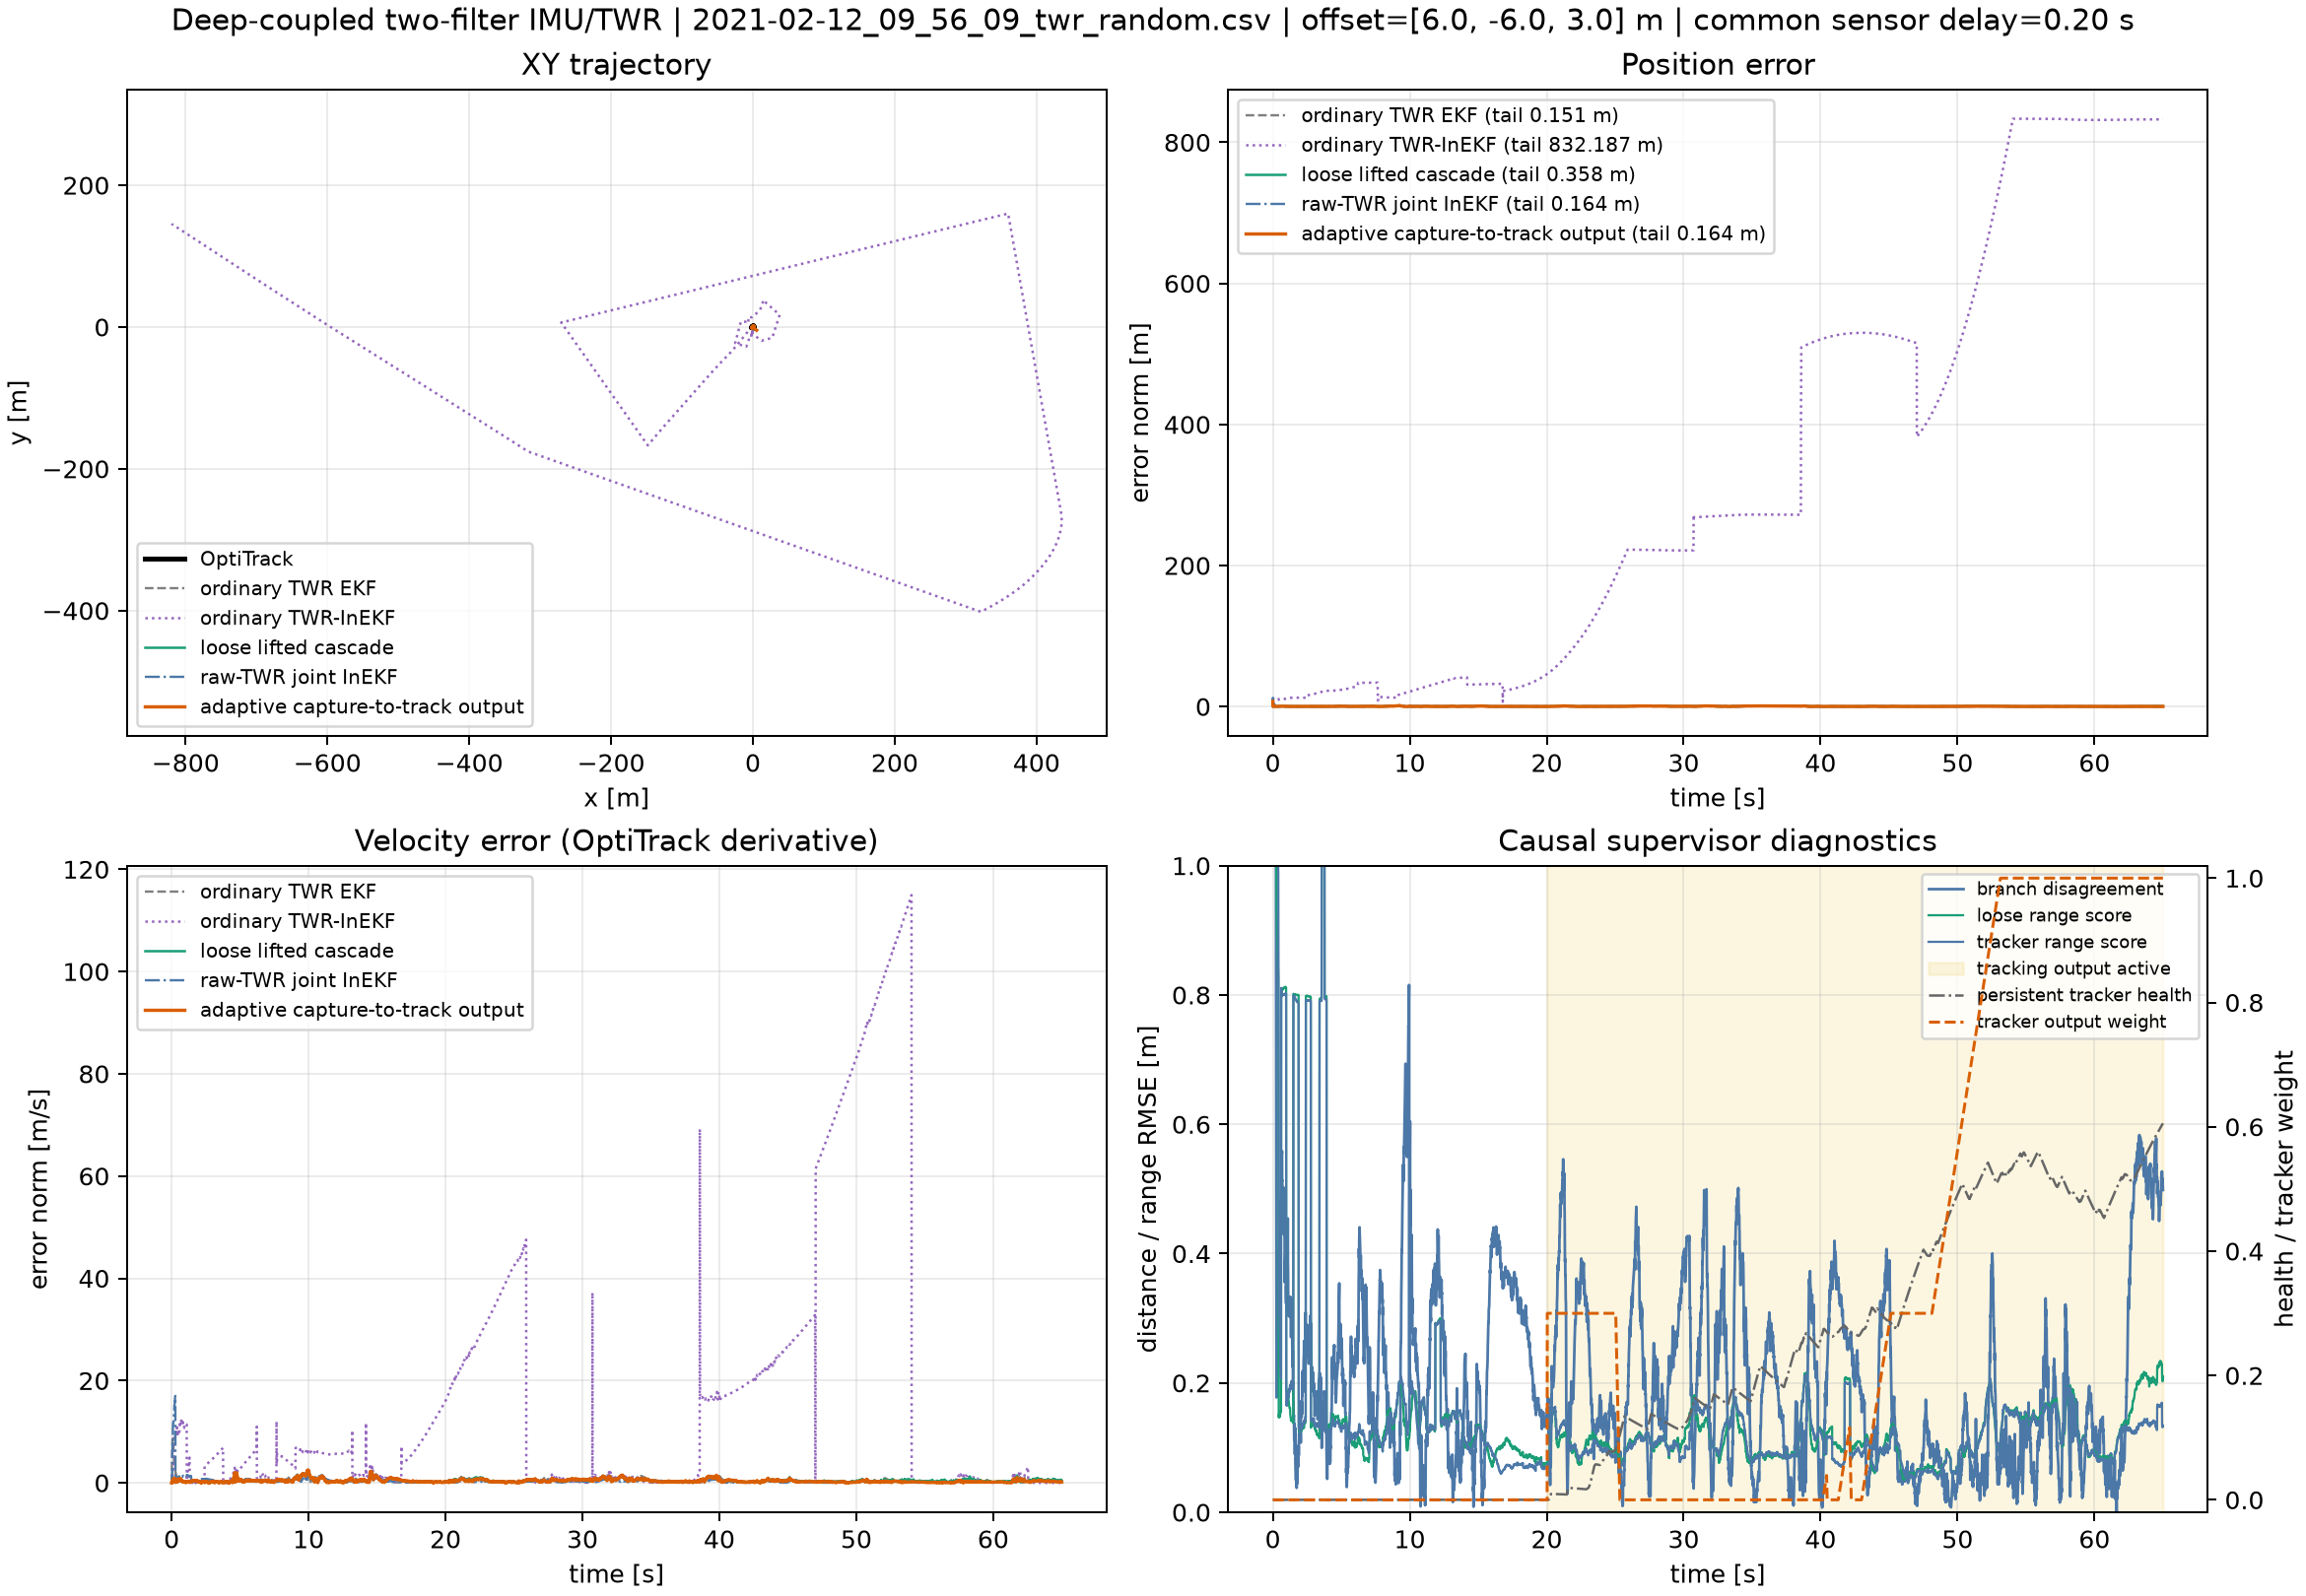
\includegraphics[width=0.98\textwidth]
{../imu-uwb-state-augment-deep-coupled-two-filters/results/deep_coupled_delay_full/real/representative/trajectory_and_errors.png}
\caption{代表性随机轨迹大初差五方法回放。普通 EKF/InEKF 与原
Task06 基线逐样本一致；背景阴影为 track 模式，监督器子图显示持续
健康度、低健康保护和 tracker 实际权重的平滑交接。}
\label{fig:representative}
\end{figure}

\subsection{大初差捕获--跟踪端到端蒙特卡洛}

旧试验总时长与强制 capture 驻留时间同为 20 s，而代码要求 $t>20$ s
后才允许切换。因此旧表中 $w(t)\equiv0$，所谓自适应输出与 capture
逐样本严格相同；该结果只能验证捕获支路，不能验证两滤波器交接。

修复后仍沿用原 Task06 的 Theodosis 类持续激励轨迹、20 Hz 总距离事件率、
$\sigma_\rho=0.1$ m，以及
$p_0\sim\mathcal U([-50,50]^3)$ m、
$v_0\sim\mathcal U([-10,10]^3)$ m/s。前 20 s 保留原单锚点大初差捕获；
随后 25 s 循环使用覆盖轨迹包围盒的固定八锚点。IMU 加入固定残余偏置
\begin{equation}
b_a^{\rm true}=[0.080,-0.056,0.040]^\top~\mathrm{m/s^2},
\qquad \hat b_a(0)=0,
\qquad \sigma_{b_a,0}=0.20~\mathrm{m/s^2},
\end{equation}
从而实际检验联合 tracker 通过传播交叉协方差校正偏置的通路。成功仍定义为
末 5 s 位置 RMSE 小于 1 m。该 45 s 有偏 IMU、多锚后段试验是端到端
监督器验证，不再与原 20 s 理想单锚捕获表偷换为同一场景。

\begin{table}[H]
\centering
\small
\caption{20 次合成大初差捕获--跟踪端到端蒙特卡洛。}
\begin{tabular}{lrrrr}
\toprule
方法 & 成功/20 & 末段位置 & 全程位置 & 末段速度\\
 & & RMSE (m) & RMSE (m) & RMSE (m/s)\\
\midrule
普通距离 EKF & 0 & 630.007637 & 383.470996 & 15.940434\\
普通 TWR--InEKF & 0 & 1857.006050 & 985.040599 & 54.653380\\
松耦合增广捕获 & 2 & 1.634523 & 10.685872 & 0.526107\\
原始 TWR 联合跟踪器 & 20 & 0.167611 & 14.018746 & 0.398315\\
自适应两滤波器输出 & 20 & 0.167611 & 10.675858 & 0.398315\\
\bottomrule
\end{tabular}
\label{tab:mc}
\end{table}

20/20 次都在中位 20.60 s 首次进入 track，末 5 s 输出均与 capture
不同且都曾达到 $w=1$；track 样本比例中位为 0.5423，平均权重中位为
0.4106。deep 相对 capture 的全程/末段位置为
20/0/0、20/0/0 次优/平/差，中位分别改善 0.010014 m 和 1.466912 m；
全程/末段速度中位分别改善 0.001859 m/s 和 0.127791 m/s，逐次为
11/0/9 和 15/0/5。末段 deep 与独立 tracker 的中位数相同是因为 20 次
末段均已全权接管；两者全程位置 10.675858 m 与 14.018746 m 不同，证明
deep 前段确实使用 capture，而不是整段复制 tracker。

\begin{figure}[H]
\centering
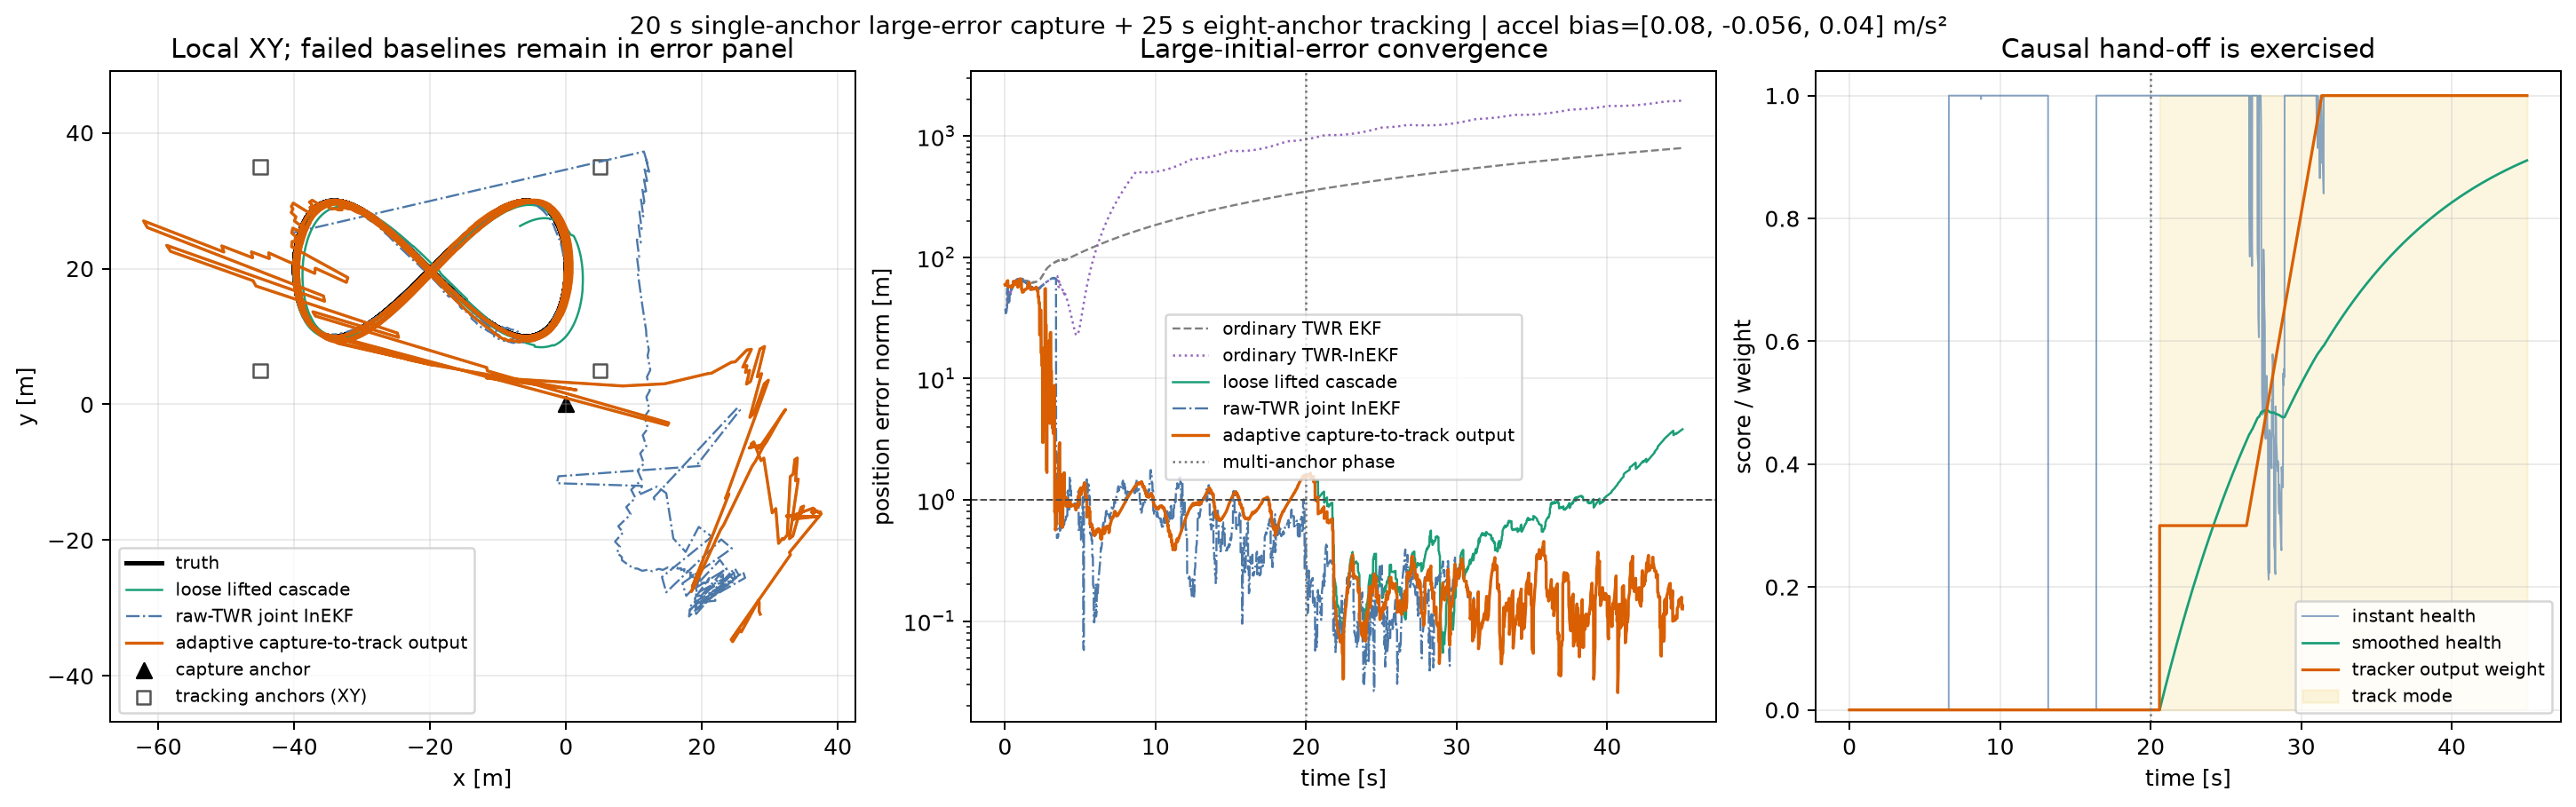
\includegraphics[width=0.94\textwidth]
{../imu-uwb-state-augment-deep-coupled-two-filters/results/deep_coupled_delay_full/synthetic/representative.png}
\caption{合成大初差端到端代表试验。前 20 s 为原单锚捕获，虚线后为
八锚跟踪；右图直接展示 track 模式、持续健康度和实际权重从 0.3 到 1
的交接。普通 EKF/InEKF 的发散保留在中间对数误差图。}
\label{fig:synthetic}
\end{figure}

\section{结论与复现}

本次保留增广捕获支路，并增加原始 TWR 通过联合协方差修正 15 维误差
状态的 InEKF tracker；离散重置、健康交接和低健康 $w=0$ 保护兼顾
大初值捕获与稳态跟踪。共同 IMU/TWR 时刻校正由距离和惯性两类证据
支持，没有只移动 UWB。补齐普通 EKF/InEKF 后，不能声称本方法在零
初差或所有尾段指标最优；可主张的是 large 初值全程位置/速度统计最好、
相对 capture 四指标零退化，且 tracker 无普通 InEKF 的五次 gate
锁死。修复后的合成端到端试验不再允许 $w\equiv0$ 平凡通过，并表明
多锚决定性量测优势可在 capture 被残余加速度偏置拖离时保留正确 tracker。
尚未解决辅助状态流形投影、逐锚 NLOS、滤波器互协方差和全局
稳定性证明；结论仅适用于当前数据及所列参数。

\begin{verbatim}
.\run_deep_coupled.ps1 -Mode test
.\run_deep_coupled.ps1 -Mode calibrate
.\run_deep_coupled.ps1 -Mode full -SyntheticDuration 45
\end{verbatim}

\section*{参考文献}
\small
\setlength{\tabcolsep}{0pt}
\noindent
\begin{tabular}{@{}p{2.1em}p{\dimexpr\textwidth-2.1em\relax}@{}}
[1] & Oursland, J. and Mehrabian, A.,
``An Invariant Extended Kalman Filter for IMU--UWB Sensor Fusion,''
IEEE RO-MAN, 2024,
\href{https://doi.org/10.1109/RO-MAN60168.2024.10731434}
{doi:10.1109/RO-MAN60168.2024.10731434}.\\[0.2em]
[2] & Theodosis, P. A., et al.,
``State Estimation for a Class of Linear Systems with Quadratic Output,''
\href{https://arxiv.org/abs/2006.02688}{arXiv:2006.02688}, 2020.\\[0.2em]
[3] & Sifour, O., Berkane, S., and Tayebi, A.,
``Cascaded Tightly-Coupled Observer Design for Single-Range-Aided
Inertial Navigation,''
\href{https://arxiv.org/abs/2512.06198}{arXiv:2512.06198}, 2025.\\[0.2em]
[4] & TU Delft, ``UWB dataset (Version 1),''
\href{https://doi.org/10.4121/14827680.v1}
{doi:10.4121/14827680.v1}.\\
\end{tabular}

\end{document}
